\subsection{Parameter selection}
\label{sec:pf_params}

Once the inherent data issues have been dealt with,
we can begin determining the values of the model parameters.
Some of these are fixed and constant across all vehicles, routes, and stops,
for example,
GPS error, $\GPSerr$,
system noise, $\Vnoise$,
and minimum dwell time, $\mindwell$.
Others will inevitably vary between routes, stops, and time of day,
such as stopping probability, $\Prstop$,
and dwell time, $\dwell$.


% We explore these by modelling a subset of routes throughout Auckland over several days,
% using historical data to allow us to vary parameters and compare their effects.
% Some parameters, notably $\GPSerr$ and $\dwell$
% can be determined from the data:
% the value $\GPSerr$ can be approximated by looking at the variability
% of points around the route,
% since we assume there is no directional bias,
% so the distance from an observation to the route is an approximate estimate
% of measurement error.


\subsubsection{GPS error}
\label{sec:pf_params_gps}

The GPS or \emph{measurement} error used in the model has a strong effect on performance, as we saw in \cref{sec:pf_issues}. We can get a simple estimate of GPS error by examining the distribution of observations around the route; that is, we computed the shortest distance between the route and each observation, and graphed the results in \cref{fig:pf_param_gps}. We see two modes at about 0.5 and 2.5~meters, which could be due to a multitude of reasons. One likely one, however, is \emph{road width}, since the route shapes typically run in the middle of the road and the buses drive either side of the center line. Single-lane roads will have a smaller average distance between the bus and the center line, while for roads with two or more lanes, this will be larger. Additionally, some roads have a median (either painted or raised) which further increases the distance between the bus and the ``center line''. It is possible that some combination of this could result in the distribution shown in \cref{fig:pf_param_gps}.



\begin{knitrout}\small
\definecolor{shadecolor}{rgb}{0.969, 0.969, 0.969}\color{fgcolor}\begin{figure}
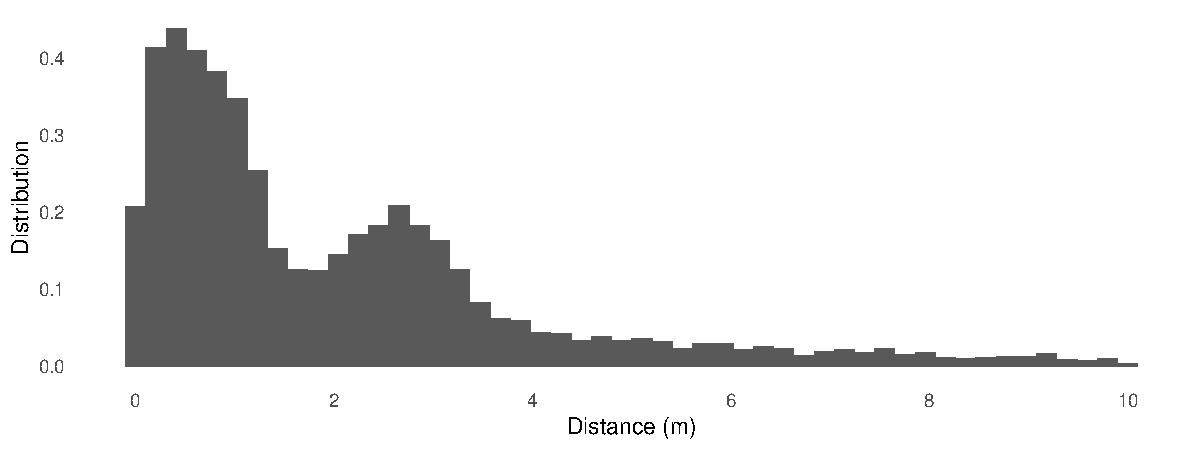
\includegraphics[width=\maxwidth]{figure/pf_param_gps-1} \caption[Distribution of distance from observation to nearest point on the route, truncated to 10~m]{Distribution of distance from observation to nearest point on the route, truncated to 10~m.}\label{fig:pf_param_gps}
\end{figure}


\end{knitrout}

The other issue is the heavy tail in the distribution of distance to path, which we trunctated to 10~meters to more easily see the modes. GPS devices usually have good accuracy, but occasionally they may be quite far off of the true location, possibly due to physical interference. 6\% of bus observations were more than 10~meters from the shape, excluding any observations greater than 50~meters since these were most likely attributed to the wrong trip (and therefore not anywhere near the route path). This would explain a large proportion of the degeneration rate (\cref{fig:model_performance_degen}), which we saw previously decreases significantly with increased GPS error.





\subsubsection{System noise}
\label{sec:pf_params_noise}

The definition of system noise is model-dependent; for transition models $f_{A1}$ and $f_{A2}$ it is \emph{the average change in speed per second}, while for model $f_{A3}$ it is \emph{the average change in acceleration per second}. From the simulations in \cref{sec:pf_issues}, we demonstrated that system noise affected the performance of the particle filter (how often resampling is required) but neither the degeneration rate nor parameter estimation.

Unlike GPS error, it is not possible to estimate system noise directly from the data. Indeed, most of the time a vehicle's speed is constant, but may change suddenly at certain locations (which are unknown), so the system noise must allow for this. We found that a smaller value of system noise under the second transition model $f_{A2}$ gave the best results in terms of sampling possible trajectories, and as such this was the model used during the simulation.



\subsubsection{Dwell times}
\label{sec:pf_params_dwell}

We are able to observe a large proportion of dwell times at stops, by compiling all those for which we have observed both arrival times $\Varr_{srm}$ and departure times $\Vdep_{srm}$ at stop $m$ of trip $r$ on day $s$ giving us a set of dwell times
\begin{equation}
\label{eq:dwell_time_obs}
\Vdwell_{srm} = \Vdep_{srm} - \Varr_{srm}
\end{equation}

\begin{knitrout}\small
\definecolor{shadecolor}{rgb}{0.969, 0.969, 0.969}\color{fgcolor}\begin{figure}
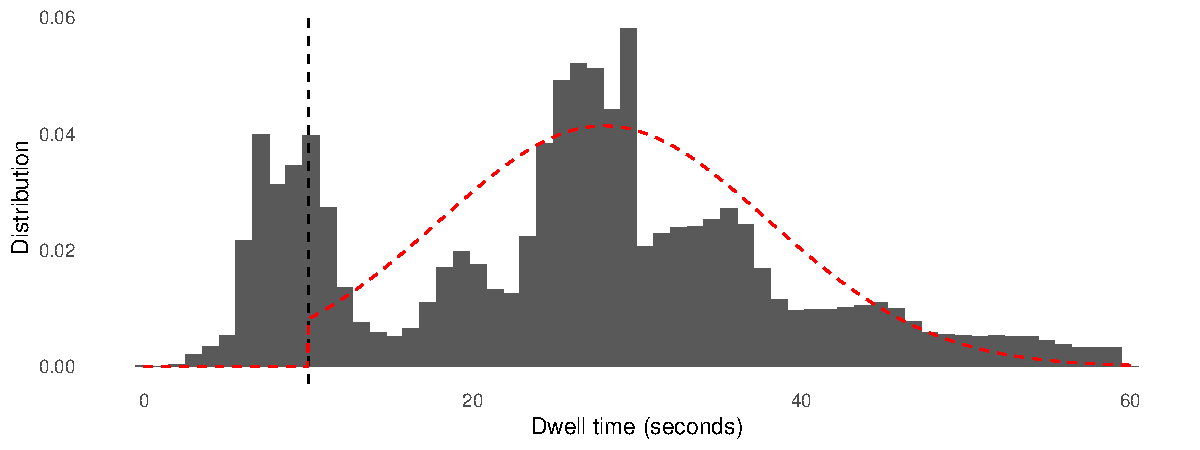
\includegraphics[width=\maxwidth]{figure/observed_dwell-1} \caption[Distribution of dwell times observed over the course of five days, truncated at one minute]{Distribution of dwell times observed over the course of five days, truncated at one minute.}\label{fig:observed_dwell}
\end{figure}


\end{knitrout}

There is no precise way to measure the minimum dwell time parameter $mindwell$. \cite{Hans_2015} used $\mindwell = 6$~seconds, which is marked by a dashed vertical line in \cref{fig:observed_dwell}. There are a few dwell times less than this, but given the spike at 6~seconds, it seems reasonable to continue with this value.

The raw data from five~days' observations are shown in \cref{fig:observed_dwell}. Here, we see an interesting pattern with apparent peaks every nine~seconds. While we could not determine the precise cause, we assume it to be due to a systematic problem in the arrival time recording system used to collect the data. From the historical dwell time data, we were able to estimate the mean and variance of dwell time for each stop $j$, $\bar\dwell_j$ and $\dwellvar_j$, respectively, which could then be used in the dwell time model.


The dwell times for each stop calcualted above \emph{include} the minimum dwell time phase. To avoid having to recompute each stop's dwell time parameter whenever $\mindwell$ is changed, we adjusted the mean of each stop's dwell time at run time to account for the minimum dwell time. That is, we use $\dwell_j = \bar\dwell_j - \mindwell$ in \cref{eq:stop_dwell_time}.
